%% prelim.tex
\section{Preliminaries}
\label{sec:prelim}
%%%%

\subsection{Basics}
We begin with basic definitions and notation following~\cite{charalampopoulos2018extended,barton2014linear,ilie2011minimum,belazzougui2015space:unusual}.
For any integers $i\le j$, we denote by $i..j$ or $[i..j]$ the \textit{discrete interval} $\set{i, i+1, \dots, j}$. For a set $A$, we denote by $|A|$ the \textit{cardinality} of $A$, by $A^*$ and $A^+$ the \textit{sets of all finite sequences} of length $\ge 0$ and length $\ge 1$ over $A$, respectively.
We assume the \textit{unit-cost RAM model} with machine word size $w = \floor{\log n}$ equipped with the standard Boolean and arithmetic operations over integers, where $n$ is an input size~\cite{cormen2009introduction}.

%%%% Strings
\subsection{Strings and factors}
Let $S = S[1]\dots S[n] \in \Sigma^n$ be a \textit{string} (or a \textit{word}) \textit{of length} $n = |S|$ over a finite \textit{alphabet} $\Sigma$ of size $\sigma$. In particular, we consider the case of an \textit{integer alphabet} $\Sigma = \set{0,1,\dots, \sigma - 1} \subseteq \set{1, \dots, n}$. We define $\Sigma(S)$ to be the alphabet of $S$. 
We often write $S[1..|S|]$ for $S$ to emphasize the indexing of $S$, meaning $S: 1..|S| \to \Sigma$. 
For two strings $x[1..m]$ and $y[1..n]$, we denote the \textit{concatenation} of $x$ and $y$ by $(x\cdot y)[1..m+n] = x[1]\dots x[m]\cdot y[1]\dots y[n]$.
For positions $i\le j$ in $S$, we denote by $S[i..j]$ the \textit{factor} (or a \textit{substring}) of $S$ that starts and ends at positions $i$ and $j$, respectively, and by $\eps$ the \textit{empty word} of length $0$. A (non-empty) prefix (resp.~a suffix) of $S$ is a factor of the form $S[1..i]$ (resp.~$S[i..n]$) for some $\btw i1n$. A factor $u$ of a string $w$ is \textit{proper} if $u\not= w$. In what follows, we denote by $\Fac(S)$ and $\Pref(S)$ the \textit{sets of all factors} and \textit{all prefixes} of a string $S$, respectively. 

%%%% Convention
Throughout this paper, we assume an \textit{input string} $S = S[1..n]$ of length $n\ge 1$ over an alphabet $\Sigma$ is given to our algorithms. For convention, we assume an extended alphabet $\hat\Sigma = \Sigma\cup\set{\sharp, \daller}$, where $\#, \daller \not \in \Sigma$. Then, we define an \textit{extended string} $\hat S[0..n+1] = \hat S[0]\cdot S[1..n]\cdot \hat S[n+1]$  over $\hat \Sigma$ of length $n+2$, whose index starts from $0$ by prepending and appending special endmarkers $\hat S[0] = \sharp$ and $\hat S[n+1] = \daller$, respectively. 
%% Under this convention, we formulate classes of patterns in terms of $\hat S$ rather than an input $S$.
%% 
A position $p \in 1..|S|$ is an occurrence of a word $w$ in $S$, if $w = S[p..p+|w|-1]$ holds. Then, we say that $w$ \textit{occurs in} a string $S$ at start position $p$ or end position $q = p + |w| - 1$. 
We denote by $\spos(w)$ and $\epos(w)$ the sets of all start positions and all end positions of $w$ in $S$, respectively. 
We define the number of occurrences of $w$ by $\occ(w) := |\spos(w)| = |\epos(w)|$. 

\subsection{unusual words}
\label{sec:unusual}
%% 
We introduce classes of unusual words of a string $S$.
A string $w \in \Sigma^*$ is \textit{trivial} if $|w| = 1$, i.e., $w = c$ for some letter $c$ in $\Sigma$, and \textit{non-trivial} otherwise.
We can easily see that any non-tivial string $w$ has length two and has the form $w = aub$ for some letter $a, b \in \hat\Sigma$ and a possibly string $u \in \Sigma^*$. Throughout, we assume $|\Sigma(S)|\ge 2$ and consider only non-trivial unusual words.
Let $S = S[1..n] \in \Sigma^n$ be a string over alphabet $\Sigma$.
For convention, we assume virtual extended string $\hat S[0..n+1] = \# S\daller \in \hat\Sigma^{n+2}$ obtained from $S$ by prepending and appending endmarkers, where $S[0] = \#$ and $S[n+1] = \daller$.

%% %%%%
%% \mysubsubsection{Classes of unusual words of a string} 
%% We introduce classes of unusual words of a string $S$. A string $w \in \Sigma^*$ is \textit{trivial} if $|w| = 1$, i.e., $w = c$ for some letter $c$ in $\Sigma$, and \textit{non-trivial} otherwise. We remark that clearly, non-tivial string $w$ has length three and has the form $w = aub$ for some letter $a, b \in \hat\Sigma$ and a non-empty string $u \in \Sigma^+$. Throughout, we consider only non-trivial unusual words.

%% %%%
%% %Ilie and Smyth~\cite{ilie2011minimum} initiated the study of
%% A \textit{minimal unique substrings} (MUSs) of a string $S$, studied by Ilie and Smyth~\cite{ilie2011minimum}, is a non-trivial string $w$ that has unique occurrence in $S$, and any proper factor has more than one occurrences in $S$. 
%% That is, a MUS of $S$ is a string $w = a u b$ with $a, b\in \hat\Sigma$ and $u \in \Sigma^+$ such that
%% \begin{enumerate*}[(i)]
%% \item $\Occ(w) = 1$; and 
%% \item $\Occ(au) \ge 2$ and $\Occ(ub) \ge 2$. 
%% \end{enumerate*}
%% We denote by $\MAW(S)$ and $\MUS(S)$ the sets of all MAWs and all MUSs of a string $S$, respectively. 

%% %%% 
%% The class of \textit{minimal rare words} was introduced by Belazzougui and Cunial~\cite{belazzougui2015space:unusual}, whose abstracted the properties of unusual words with statistical surprise studied by Apostolico, Bock, Lonardi, and Xu~\cite{apostolico2000efficient}. 
%% For every $k\ge 0$, a \textit{$k$-minimal rare word} ($k$-MRW) of a string $S$ is a non-trivial string $w$ that occurs in $S$ exactly $k$ times, and any proper factor occurs in $S$ less frequently (see \cite{belazzougui2015space:unusual}). That is, a $k$-MRW of $S$ is a string $w = a u b$ with $a, b\in \hat\Sigma$ and $u \in \Sigma^+$ such that
%% \begin{enumerate*}[(i)]
%% \item $\Occ(w) = k$; and 
%% \item $\Occ(au) \ge k+1$ and $\Occ(ub) \ge k+1$. 
%% \end{enumerate*}
%% We denote by $\MRW_k(S)$ and $\MRW(S) = \bigcup_{k\ge 0} \MRW_k(S)$ the sets of all $k$-MRWs and all MRWs of a string $S$, respectively. 

%% %%%% 


%% \subsection{Texts, substrings, prefixes, and suffixes}
%% %%%%
%% We assume the word RAM model with machine word size $w = \floor{\log n}$ with input size $n$~\cite{navarro2016cds:book}, where space is always measured in machine \textit{words}, not \textit{bits}. 
%% For any integers $i\le j$, we define intervals $[i]=\set{1,\dots,i}$ and $[i..j] = \set{i, i+1, \dots, j}$.

%% Let $\Sigma$ be an alphabet of $\sigma\ge 2$ characters. We denote by $\eps$ the \textit{empty string} of length $0$, and by $\Sigma^*$ the set of all strings of length $\ge 0$. 
%% Throughout this paper, as input, we always assume a fixed string $S[1..n] = S[1]\dots S[n] \in \Sigma^*$ of length $|S| = n$ over $\Sigma$, called a \textit{text}, where an index starts from $1$. The string is terminated by a special endmarker $S[n]=\daller$, which do not appear elsewhere in $S$, and are smaller than any other characters. $S\rev$ denotes the \textit{reverse} of $S$, i.e., $S\rev = S[n]\dots S[1]$. 
%% If $S = XYZ$ for some strings $X, Y, Z \in \Sigma^*$, we call $X, Y$, and $Z$ a \textit{prefix}, a \textit{substring} and a \textit{suffix} of $S$, respectively.
%% For $1\le p \le q\le n$, $S[p..q]$ denotes the substring of $S$ starting from position $p$ and ends at $q$. Then, $p$ and $q$ are called the \textit{start-position} and \textit{end-position} of $W$.
%% For any string $W \in \Sigma^*$, $\spos[S](W)$, $\epos[S](W)$, and $\occ[S](W) = |\spos[S](W)| = |\epos[S](W)|$  denote the set of all start-positions, the set of all end-positions, and the number of occurrences of $W$ in $S$, respectively.
%% In what follows, we will omit the subscript $S$ if it is clear from context.


%% %% %%%%%%
%% %% %% size: n=12
\begin{table}[t]
\caption{
  The set of lexicographically ordered suffixes of a string \texttt{abcadabcabc\daller} of length $n=13$, where $\# < \daller < a < b < c < d$ and the index starts from $0$. 
}
\ttfamily
\centering 
\begin{tabular}{wc{2.5em}wc{2.5em}wc{2.5em}wc{2.5em}lcccc}
%% \hline
\toprule
rank	& SA	& BWT	& LCP		& suffix	\\
\midrule
0	& 0	& \$	& 0		& \#abcadabcabc\$	\\
1	& 12	& c	& 0		& \$	\\
2	& 9	& c	& 0		& abc\$	\\
3	& 6	& d	& 3		& abcabc\$	\\
4	& 1	& \#	& 4		& abcadabcabc\$	\\
5	& 4	& c	& 1		& adabcabc\$	\\
6	& 10	& a	& 0		& bc\$	\\
7	& 7	& a	& 2		& bcabc\$	\\
8	& 2	& a	& 3		& bcadabcabc\$	\\
9	& 11	& b	& 0		& c\$	\\
10	& 8	& b	& 1		& cabc\$	\\
11	& 3	& b	& 2		& cadabcabc\$	\\
12	& 5	& a	& 0		& dabcabc\$	\\
\bottomrule
\end{tabular}
\end{table}


%% %% size: n=12
%% \begin{table}[t]
%% \caption{
%%   An example of the rank, suffix, inverse suffix, and Burrows-Wheeler Transformation (BWT), and longest common prefix arrays, and the set of lexicographically ordered suffixes of a string \texttt{abcadabcabc\daller} of length $n=13$, where $\# < \daller < a < b < c < d$ and the index starts from $0$. 
%% }\label{tbl:arrays}
%% %% \small 
%% \ttfamily
%% \renewcommand{\arraystretch}{.8}
%% \centering
%% \smallskip
%% \begin{tabular}{wc{2.5em}wc{2.5em}wc{2.5em}wc{2.5em}lcccc}
%% %% \hline
%% \toprule
%% rank	& SA	& BWT	& LCP		& suffix	\\
%% %% index from one 
%% %% \midrule
%% %% 1	& 1	& \$	& 0		& \#abcadabcabc\$	\\
%% %% 2	& 13	& c	& 0		& \$	\\
%% %% 3	& 10	& c	& 0		& abc\$	\\
%% %% 4	& 7	& d	& 3		& abcabc\$	\\
%% %% 5	& 2	& \#	& 4		& abcadabcabc\$	\\
%% %% 6	& 5	& c	& 1		& adabcabc\$	\\
%% %% 7	& 11	& a	& 0		& bc\$	\\
%% %% 8	& 8	& a	& 2		& bcabc\$	\\
%% %% 9	& 3	& a	& 3		& bcadabcabc\$	\\
%% %% 10	& 12	& b	& 0		& c\$	\\
%% %% 11	& 9	& b	& 1		& cabc\$	\\
%% %% 12	& 4	& b	& 2		& cadabcabc\$	\\
%% %% 13	& 6	& a	& 0		& dabcabc\$	\\
%% %% \bottomrule
%% %%
%% %% index from zero
%% \midrule
%% 0	& 0	& \$	& 0		& \#abcadabcabc\$	\\
%% 1	& 12	& c	& 0		& \$	\\
%% 2	& 9	& c	& 0		& abc\$	\\
%% 3	& 6	& d	& 3		& abcabc\$	\\
%% 4	& 1	& \#	& 4		& abcadabcabc\$	\\
%% 5	& 4	& c	& 1		& adabcabc\$	\\
%% 6	& 10	& a	& 0		& bc\$	\\
%% 7	& 7	& a	& 2		& bcabc\$	\\
%% 8	& 2	& a	& 3		& bcadabcabc\$	\\
%% 9	& 11	& b	& 0		& c\$	\\
%% 10	& 8	& b	& 1		& cabc\$	\\
%% 11	& 3	& b	& 2		& cadabcabc\$	\\
%% 12	& 5	& a	& 0		& dabcabc\$	\\
%% \bottomrule
%% \end{tabular}
%% \end{table}
%% %%%%%%%%%%


%%\subsection{Array-like text indexing data structures}
%%\label{sec:prelim:ds:array}
%%%%%%%%%%5
%% Let $S = S[1..n] \in \Sigma^n$ be a string of length $n$ (denoted \textsc{Txt}) throughout.
%% We assume that the reader is familier with fundamental text indexing data structures such as the suffix tree. Below, we introduce basic text indexing array structures.  (See text books, e.g., Gusfield~\cite{gusfield1997book:stree} and Crochemore and Rytter~\cite{crochemore2002jewels} for the suffix tree and the CDAWG, and Navarro~\cite{navarro2016cds:book} for compact array-like text indexing data structures.) 


%%%%%%
\begin{figure}[t]
\centering  
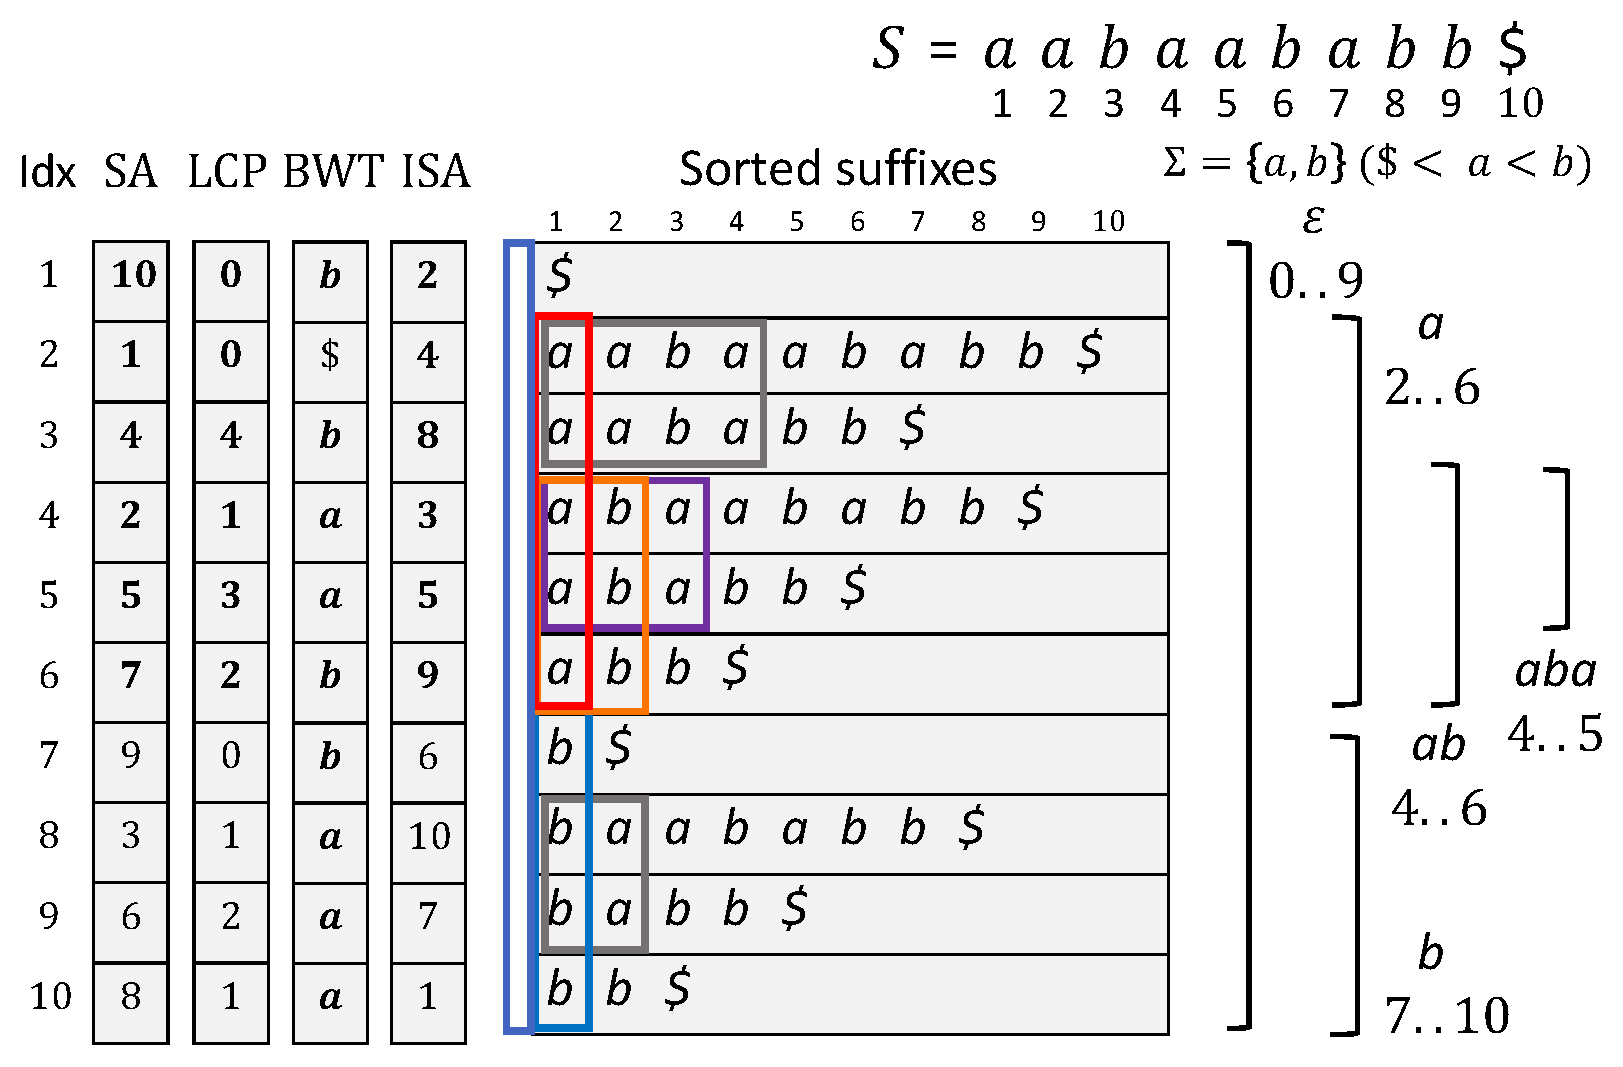
\includegraphics[width=0.70\textwidth]{fig1.pdf}
\vspace{.5\baselineskip}
\caption{An example of indexing arrays of a string $S[1..10] = aabaababb\daller$ of length $n = 10$ over alphabet $\Sigma = \set{a, b}$, whose index starts at $0$, where the left endmarker $S[0]=\#$ and the related suffixes are omitted. 
  Inside and to the right of the panel for sorted suffixes, each bold rectangle $R = [i..j]\times [0..\ell-1]$ and square bracket
indicate a rich representation $(i..j, \ell)$ of a repeat of $S$ and 
the associated SA-interval $i..j$, respectively. 
%% In the panel for sorted suffixes, each bold rectangle $R = [i..j]\times [0..\ell-1]$ in the panel indicates a rich representation $(i..j, \ell)$ of a repeat of $S$, while each square bracket indicates the associated SA-interval $i..j$. 
}\label{fig:example:arrays}
\end{figure}
%%%%%%

\subsection{Text indexing arrays}
%%\label{sec:prelim:ds:array}
Let $S[1..n-1]$ be a string of length $n-1$ and $\hat S[1..n] = S\cdot \daller$ be its extended string with endmarker $\daller \not\in \Sigma$. For any position , we denote by $\Suf[p] = S[p..n]$ the suffix of $S$ starting at position $\btw i1n$. 
We introduce a set of arrays for indexing a string as follows (see~\cite{navarro2016cds:book} for details).
We refer to lexicographic ranks as $i, k$ and positions as $p, q$.


The \textit{suffix array} $SA$ and \textit{inverse suffix array} $ISA$~\cite{manber:myers1993suffixarrays} are integer arrays defined as follows. 
The array $SA$ contains all suffixes of $\hat S[1..n]$ sorted in the increasing lexicographic order $<_\lex$ such that 
$S[SA[1]..n]<_\lex \dots <_\lex S[SA[n]..n]$. that is, $SA[k] = p$ means that $p = SA[k]$ is the starting position of the $k$-th rank in $<_\lex$ in $S$. 
Then, $ISA$ represents the inverse function of $SA$ such that $SA[ISA[p]] = p$ for all $p \in [n]$.

In the \textit{rich representation} on $SA$ array (see, e.g.\cite{kasai:lee2001lcp:linear,abouelhoda2004replacing}), we can uniquely encode any factor $w$ of a string $S$ by a triple $\tau = (i, j, \ell)$, denoted by $(i..j, \ell)$, such that
\begin{enumerate*}[(i)]
\item $i..j \subseteq 1..n$ is the SA-interval of $w$, i.e., $SA[i..j] = \Occ(w)$; and  
\item $\ell$ is the length of $w$, i.e., $\ell = |w|\ge 0$. 
\end{enumerate*}
Conversely, the rich representation $\tau = (i, j, \ell)$ can be decoded by the function $\getfactor(i..j, \ell) := S[p..SA[k]+\ell-1]$ using $\SA$ and $S$, where $\btw kij$ can be any rank in $i..j$. 

The \textit{longest common prefix array} $LCP[1..n]$ contains in the $k$-th rank the length of the longest common prefix of adjuscent suffixes $\Suf[SA[k-1]]$ and $\Suf[SA[k]]$ for all $k \in [n]$; We define $LCP[1] = 0$. It can be preprocessed in linear time supporting the \textit{range minima query} $RMQ_{LCP}(i, j)$ that, given $i\le j$, returns the minimum of $\set{\LCP[i], \LCP[i+1], \dots, \LCP[j]}$ in constant time and $O(n)$ space (Bender and Colton~\cite{bender:colton2000thelcaproblem}).
An example is shown in \cref{fig:example:arrays}. 

%%%
The \textit{Burrows-Wheeler Transformation} $\BWT[1..n]$ defines the permutation of a string $S$ by $BWT[k] = S[SA[k]-1]$ for all $k \in [2..n]$; We let $BWT[k] = \daller$ with $SA[k] = 1$~\cite{burrows:wheeler1994blocksorting}. 
%% For any $k \in [n]$, the \textit{LF-mapping} is defined by $LF(k) = ISA[n]$ if $SA[k]=1$ and $LF(k) = ISA[SA[k]-1]$ otherwise.
%%
It can be preprocessed in linear time in the \textit{Wavelet Tree} data structure (by~\cite{grossi2003high}) supporting the \textit{range distinct query} $RDQ_{BWT}(i, j)$ that, given $i\le j$, returns the set of mutually distinct characters in the range $BWT[i..j]$ in $O(\log\sigma)$ time and
linear space. 
%% $O(n/\log_\sigma n)$ space.
All the arrays can be constructed from $S$ in linear time over integer alphabet (see the textbook~\cite{navarro2016cds:book}). 


%% %%%%% 
%% \subsection{A concise representation of a substring}
%% \label{sec:triple}
%% We introduce a concise representation of a substring $W$ of a string $S$ with constant size, called the \textit{rich representation}, or simply a \textit{triple}, as follows~\cite{kasai:lee2001lcp:linear,ohlebusch2013bookbioinfo,belazzougui2015space:unusual}. 
%% Suppose that $SA \in [n]^n$ is the suffix array of $S$. Let $W \in Substr(S)$ be any substring of $S$. We can easily see that all ranks $k\in [1..n]$ whose starting positions $SA[k]$ belong to $\spos(W)$ occupy the contiguous subinterval $[L..R]\subseteq [1..n]$. We call this range $[L..R]$ the \textit{SA-range} of $W$.
%% We define the \textit{triple} for $W$ to be the integer triple $\tau = (L, R, \ell) \in [n]^3$, denoted $([L..R], \ell)$, such that $[L..R]$ is the SA-range of $W$ and $\ell = |W|$ is the length of $W$.
%% Conversely, $\tau$ \textit{defines} $W$ if $W = S[p..p+\ell-1]$ with $p = SA[L]$ is well-defined for some $k \in [L..R]$, and is unique. 
%% %%% 
%% For example, in \cref{tbl:arrays}, the substring $\mathtt{bc}$ has the triple $([7..9], 2)$ since it has the SA-range $[7,9]$ in $SA[1..13]$ and has the length $|W|=2$.


%% %%%% 
%% \mysubsubsection{Maximal repeats}
%% %%%%
%% To realize efficient enumeration of classes of unusual words, we use the class of maximal repeats of a string $S$, defined as follows.
%% Let $S = S[1..n] \in \Sigma^n$ be a string over alphabet $\Sigma$ and $\hat S[0..n+1] = \# S\daller \in \hat\Sigma^{n+2}$ be its extended version with endmarkers.
%% Let $u \in \Sigma+$ be any factor of $\hat S$. Since $\#, \daller \not\in \Sigma$, we see $u \in \Fac(S)$, namely, $u$ is contained in the content $S$.

%% \begin{definition}[maximal repeat]\rm 
%% A string $u \in \Sigma+$ is a \textit{maximal repeat} of $S$ if it satisfies conditions (1) and (2) below: 
%% \begin{enumerate}[(1)]
%% \item $u$ is a factor of $S$, i.e., $u \in \Fac(S)$. 
  
%% \item there exist two start positions $p, q \in \Spos[S](u)\;(p\not= q)$ of $u$ such that
%%   \begin{enumerate}[(i)]
%%   \item $u$ is \textit{left-branching} meaning that the preceding characters are mutually different, i.e., $S[p-1] \not= S[q-1]$, 
%%  and
%%   \item $u$ is \textit{right-branching} meaning that the following characters are mutually different, i.e., $S[p+|u|] \not= S[q+|u|]$. 
%%   \end{enumerate}
%% \end{enumerate}
%% \end{definition}

%% By definition, any maximal repeat $w$ occurs at least twice in $S$, that is, $w$ is a \textit{repeat} in $S$.
%% For later use, we define some notation: $\LSigma(u) \subseteq \Sigma$ (resp.~$\RSigma[](u)$) to be the sets of the preceding characters $S[p-1] \in \hat\Sigma$ (resp.~the following characters $S[p+|u|] \in \hat\Sigma$) by one over all positions $p\in \Spos(u)$ of $u$ in $\hat S$.
%% If it is clear from context, we write $\LSigma[](u)$ and $\RSigma[](u)$ for $\LSigma(u)$ and $\RSigma(u)$ by omitting subscript $\hat S$, respectively. 
%% In this notation, we see that a nonempty string $u$ is a maximal repeat of $S$ if and only if (1) $u \in \Fac(S)$ and (2) $|\LSigma(u)| \ge 2$ and $|\RSigma(u)| \ge 2$.


%% Now, we define the class of maximal repeats. 
%% %%are one of the most fundamental features in a string. 
%% Any subword $W$ of $S$ is called a \textit{repeat} if it occurs at least twice in $S$, namely, $\occ(W) \ge 2$.
%% A repeat $W$ is said to be \textit{left-branching} (resp.~\textit{right-branching}) in $S$ if either 
%% (i) $W$ is a prefix  of $S$ (resp.~a suffix of $S$), or 
%% (ii) there exist a pair of distict characters $a\not= b$ in $\Sigma$ such that $\occ(aW) \ge 1$ and $\occ(bW) \ge 1$ (resp.~$\occ(Wa) \ge 1$ and $\occ(Wb) \ge 1$).
%% A \textit{maximal repeat} is any repeat $W$ in $S$ that is both right-branching and left-branching in $S$. In what follows, $MR(S)$ denotes the set of all maximal repeats in $S$, and $\mu(S) = |MR(S)|$ denotes their number. 

%% A \textit{left-extension} (resp.~a \textit{right-extension}) of a maximal repeat $W \in MR(S)$ is any substring of $S$ in the form $cW$ (resp.~$Wc$) such that $\occ(cW)\ge 1$ for some $c \in \Sigma$. We denote by $e_L(S)$ (resp.~$e_R(S)$) the number of the left-extensions (resp.~right-extensions) in $S$. 
%% For a substring $W$ of $S$, $[W]^S_L = \sete{ U \in Substr(S) \mid \spos(U) = \spos(W) }$ denotes the equivalence class with the representative $W$, and $\rext W$ denotes the unique longest string in $[W]^S_L$. By symmetry, we can define the equivalence class $[W]^S_R$ and the representative $\lext W$  related to $\epos(W)$.
%% We often write, e.g., $e_L$ and $[W]_L$ for $e_L(S)$ and $[W]^S_L$, by omitting $S$. 

%% \begin{remark}
%% Weobserve the following properties: 
%% (i) for any repeat $W$, $\rext W$ is a right-branching repeat, while $\lext W$ is a left-branching repeat in $S$;
%% (ii) the operators $\set{\lext\cdot, \rext\cdot}$ are
%% %associative,
%% commutative and idenpotent.  
%% %the identities $\rext{(\lext W)} = \lext{(\rext W)} =: \mext W$,  $\lext{(\lext W)} = \lext W$, and  $\rext{(\rext W)} = \rext W$. 
%% (iii) a substring $U$ is a maximal repeat if and only if there exists a substring $W$ such that $U = \mext W := \rext{(\lext W)} = \lext{(\rext W)}$.
%% \end{remark}

%% Raffinot~\cite{raffinot2001maximal} found that the set $MR(S)$ coincides to the vertex set of the CDAWG~\cite{blumer1987complete} for a string $S$. 
%% Thus, $e_R$ satisfies $\mu \le e_R \le n$ and $\sigma \le e_R \le n$~\cite{blumer1987complete,raffinot2001maximal}. 
%% Belazzougui~\textit{et al.}~\cite{belazzougui:cunial:gagie:prezza:raffinot2015composite} have focused on $e_R$ as a fundamental repetitiveness measure related to $MR(S)$, and showed that $r \le e_R$ and $z \le e_R$. In general, $e_R = \Theta(n)$, while $e_R$ can be much smaller than $n$ for highly-repetitive strings. Radoszewski et al.~\cite{radoszewski:rytter2012structure:cdawg:thuemorse} showed that $e_R = O(\log n)$ for morphic strings, e.g.~Thue-Morse words.
